% !TeX root = ../thuthesis-example.tex

\chapter{基于区域索引区块链的出租车调度系统复现}
本章的主要内容是实现基于区域索引的树状区块链的出租车调度系统的复现工作;目前该课题已实现的出租车调度系统,利用geohash编码存储地图数据,实现并部署了有路径规划以及车辆匹配的算法合约,并且使用Vue 2.JS作为前端可以表现出乘客与车辆的操作界面。其中用户可以通过实时地图信息获得自己的位置以及附近在线的乘客、司机等信息。乘客在发出乘车请求后,系统自动匹配附近的符合要求的车辆信息,司机在接到订单信息后,可以选择是否接受订单。司机接受订单后,进行路径规划。当车辆接到乘客时,乘客可以选择上车,而司机则是确认到达乘客上车地点。在抵达乘客目标后,乘客需要支付订单,确认订单支付后,调度系统完成。

复现工作大致分为两步:第一步是实现区域索引区块链的出租车调度系统的复现工作,该复现工作主要基于万琦玲前辈的复现手册进行。第二步则是进一步实现基于树状区块链的区域索引出租车调度系统。

实验复现的过程,笔者已形成操作文档放入毕设仓库当中,供后来者参考。
 
本章节大致介绍一下复现的流程,主要内容为笔者在这一复现过程中所遇到的问题与解决方案,以及笔者对复现文档做出的改进与调整。当下的复现文档相较于初版大大提高了可理解性与可扩展性。

\section{区域索引区块链的出租车调度系统}

\subsection{环境配置}

操作系统 Ubuntu 22.04.1 LTS

虚拟机 VMWare Workstation Pro 17
	
一些JavaScript库:npm、truffle、node.js、ethereum、web3.js等 

区域索引区块链的二进制可执行文件(代码仓库中的 geth1 二进制可执
行文件)存放到/usr/local/bin 文件夹下

\subsection{实验步骤}

实验复现的过程,笔者已形成操作文档放入毕设仓库当中:

具体可以参考从《1 传统区块链初始化和启动》到《7 调度系统复现实验》的这一过程,其中本节重点说一下《7 调度系统复现实验》的过程,其余实验均为调度系统复现工作的前置测试实验,用于理解并测试系统的相关功能所用。

\subsubsection{初始化并启动区域索引区块链}

首先配置genesis.json,配置创世块文件,之后,命令行运行如下指令实现初始化区块链并启动区块链:

\begin{verbatim}
// 初始化区块链
geth1 --identity "MyEth" --rpc --rpcaddr 127.0.0.1  
--rpcport "8545" --rpccorsdomain "*" --datadir gethdata 
--port "30303" --nodiscover --rpcapi "eth,net,personal,web3"
--networkid 91036 init genesis.json
// 启动区块链
geth1 --datadir ./gethdata --networkid 91036 --port 
30303 --rpc --rpcaddr 127.0.0.1 --rpcport 8545 --rpcapi 
'personal,net,eth,web3,admin' --rpccorsdomain='*' --ws 
--wsaddr='localhost' --wsport 8546 --wsorigins='*' --wsapi 
'personal,net,eth,web3,admin' --nodiscover --allow-insecure-
unlock --dev.period 1 --syncmode='full' console
\end{verbatim}

指令参数解读:


\begin{itemize}
    \item identity "MyEth":	设置节点的标识。
    \item rpc:					启用RPC服务器。
    \item rpcaddr 127.0.0.1:	指定RPC服务器的IP地址。
    \item rpcport “8545”:		指定RPC服务器的端口号。(外部程序可以使用该端口接入区块链,进而借助 JSON-RPC API 或者 web3.js 库和区块链进行交互。)
    \item datadir gethdata:	指定链上数据存储目录。
    \item port “30303”:		指定节点端口号。
    \item rpcapi “eth,net,personal,web3”:启用RPC API。
    \item networkid 91036:		指定网络ID。
    \item init genesis.json:	使用genesis.json文件初始化区块链。
\end{itemize}


启动区块链后,终端中将出现 JavaScript 控制台,可以使用 JavaScript 编程语言的一个子集和链进行交互。

此时,区块链已经启动完毕,可以在控制台创建账户并进行测试;需要注意的操作有:1. 创建账号后,需要将账户信息添加到genesis.json的alloc字段中,同时赋予创建的账号初始余额,以方便后续的调度实验的进行;2. 每次启动区块链都要解锁账户,否则账户无法部署合约,进而系统无法工作

在打开的控制台中输入exit退出控制台,然后删除目录./gethdata/geth。随后,再运行一次初始化区块链和启动区块链的代码,此操作是为了强制重新加载创世块文件。此时,所有账户应该都有余额了。可以用eth.geBalance(账户地址)来检查余额,余额显示正常则表明区块链已成功建立。

\subsubsection{部署合约}

这一步,笔者并未遇到什么问题,主要介绍一下系统所用到的两个合约:

StoreMap.sol:主要有存储各种地图数据的数据结构以及查询方法,此外还提供了A-Star寻路等算法的实现

StoreTraffic.sol:主要提供了司机和乘客的各项信息的管理,导航结果,以及基于geohash的对于调度车辆的查询算法

在部署合约的这一步操作中,源复现文档仅给出了合约编译后的abi以及bytecode内容,笔者在文档中添加了Remix Desktop编译合约并记录编译结果中的ABI字段并进行进行压缩转义,同时记录bytecode(下称字节码)字段的这一过程。

将二者复制到部署合约的代码模板中,并将两份编辑好的模板复制到正在运行 geth1 的 JavaScript命令行后,合约部署的请求就已经提交至交易池。开始挖矿并密切观察控制台输出,直至获取合约地址后,说明合约部署成功。

\subsubsection{上传地图}

这一步是直接调用了现有系统的上传地图的JavaScript 脚本文件,注意需要修改StoreMap的合约地址,初始的执行数据提交的账号的公钥地址,以及要上传的地图数据文件(可选,在后续实验中修改了地图数据文件)运行该脚本,直至终端输出“地图数据上传完成”字样后,结束挖矿。此时,地图数据便已成功的上传到了区块链上。

\subsubsection{更改文件以加入账户信息}

\verb|investigation-cjzhuang2020/cjz_underg_2021_09|

按照文档说明,在仓库的路径下,找到如下文件:
乘客账户文件,车辆账户文件,StoreMap合约地址文件StoreTraffic合约地址文件,乘客的位置信息文件(包括乘客的账户信息,初始位置,调度起点,调度终点),以及车辆的位置信息文件(包括车辆的账户信息,车辆的初始位置)

将上述文件进行修改后,即可启动测试

\subsubsection{启动实验}

启动挖矿,新建两个终端,准备启动车辆客户端和乘客端的测试脚本。
\verb|python3 vehicle_test.py|
\verb|python3 passenger_test.py|

看到如下提示,说明车辆位置上传成功:

\begin{figure}
	\centering
	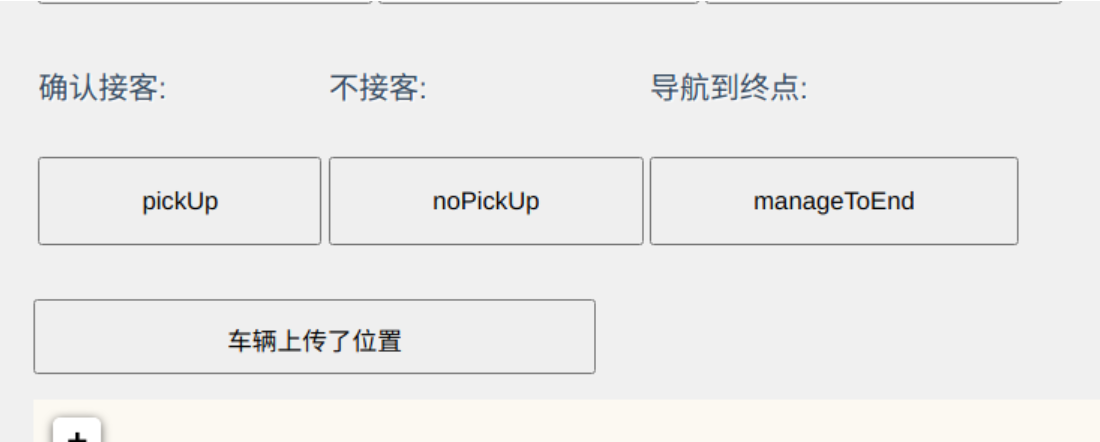
\includegraphics[width=\textwidth]{figures/车辆.png}
	\caption{车辆}
	\label{fig:车辆}
\end{figure}

被selenium控制的浏览器会进行一系列的操作,当司机端询问:Whether to pick up the passenger时,点按下图的pickUp按钮接起乘客,即可完成后续的调度步骤:

\begin{figure}
	\centering
	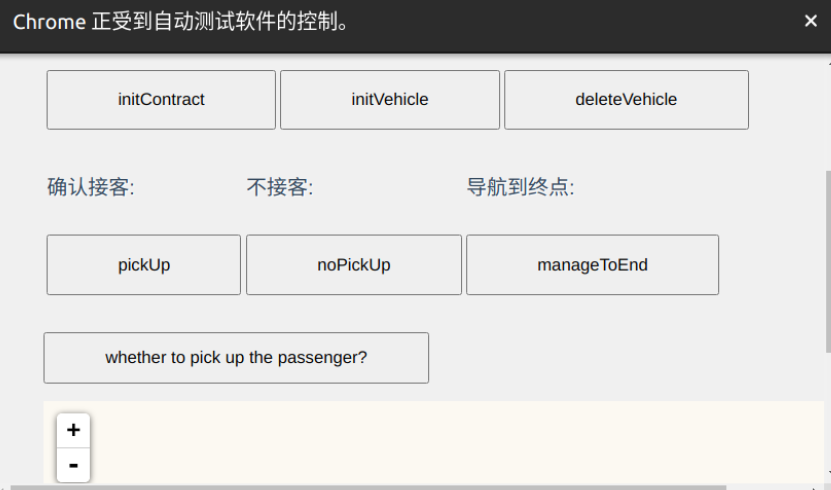
\includegraphics[width=\textwidth]{figures/车辆1.png}
	\caption{车辆1}
	\label{fig:车辆1}
\end{figure}

最终,乘客被送达目的地,并在支付订单之后乘客端的测试程序结束运行:

\begin{figure}
	\centering
	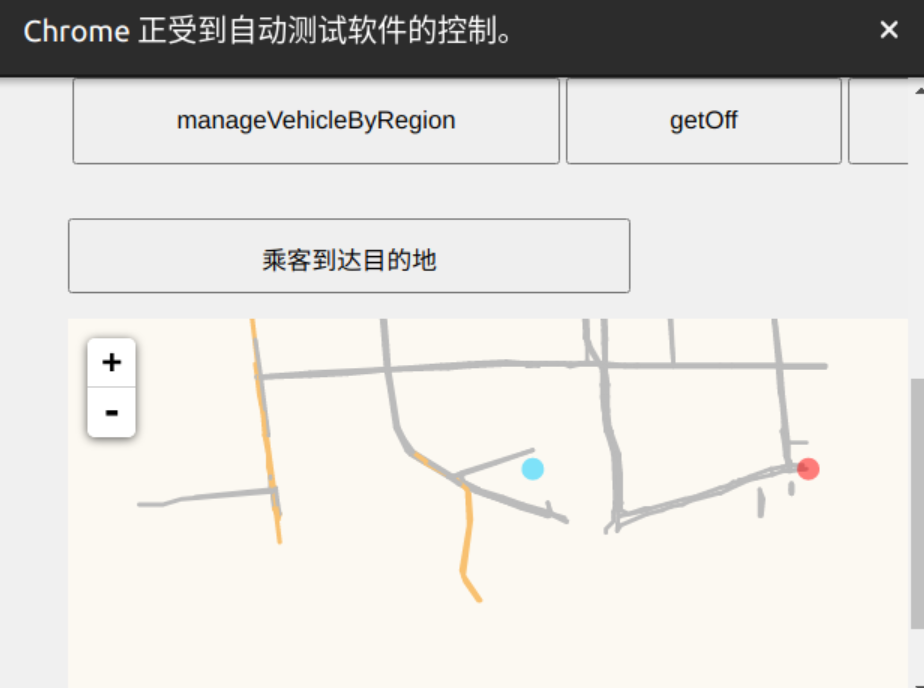
\includegraphics[width=\textwidth]{figures/车辆2.png}
	\caption{车辆2}
	\label{fig:车辆2}
\end{figure}

\section{区域索引的树状区块链的出租车调度系统}

上面的实验是在一条链上进行的复现实验,主要基于geth1进行,而本实验是实现区域索引的树状区块链的复现实验基于geth-tree完成。
	
大体操作基本同上,详情参见仓库里的《10 部署在geth-tree上的出租车调度系统复现实验》文档,这里主要介绍一下不同于上面实验的操作。

启动过程和原来的一致,只是启动文件根据区块链的不同有所变化,主要是regionid和position的变化。对于不同的账户而言,所处不同的子链,其对应的regionid和position也应不同,此外,为了支持对应的实验进行,还上传了全新的地图数据文件,参见仓库:

\section{问题及解决方案}

原版的复现手册中有着许多未说明清楚的部分,此外,操作步骤也并不完整。本小节主要介绍笔者在复现过程中遇到的问题以及解决方案。

\subsection{节点连接的问题}

笔者在进行多节点连接时,起初报错信息为终端报错,即无法同时运转两个账户,且两个账户之间,经过观察net.peerCount为0发现二者之间并未连接。

解决方案:复现手册中所说的需要把把Node1中的Key文件复制到Node2中。实际并不明确,事实上,将gethdata/keystore文件夹下的内容复制过去,则表明二者之间有着相同的账户信息,因此,初始的创世块中也应初始化相同的账户余额。笔者将两个文件夹中的genesis.json信息同步后,将Node1文件夹下的keystore文件夹复制到Node2中。
	
此时节点相互连通,问题解决。

\subsection{合约有关问题}

原版复现手册中仅仅给出了部署合约的模版代码,并未对其进行说明,此外也未对合约编译后的abi以及bytecode内容进行说明,笔者在文档中添加了Remix Desktop编译合约并记录编译结果中的ABI字段并进行进行压缩转义,同时记录bytecode(下称字节码)字段的这一过程。

\subsubsection{编译合约}

笔者使用Remix Desktop、和truffle两种方式实现了智能合约的编译。

首先是Remix Desktop,编译完成后,切换到编译选项界面,点击“Compilation Details”按钮,即可观察编译结果的详细信息,获得编译结果后,需要提取其中的应用程序二进制接口(ABI)和以太坊虚拟机字节码(bytecode)信息,需要妥善记录保存。然后是truffle,需要配置对应版本的truffle,然后在命令行中运行编译即可得到编译结果。

\subsubsection{合约的应用}

在终端中实现智能合约的调用,需要特别关注对应的区块链网络端口以及需要获取对应的contractAbi文件,在修改完合约之后要及时更新对应的contractAbi文件,否则合约会调用失败。

此外,在部署合约时,还需要注意在将合约上转至对应的区块链上时,send的信息需要position满足位于当前的子链管辖范围之内,矿工在处理交易信息时,会提取出其中所包含的position信息,若判断不满足当前位置范围,则拒绝交易。

\section{本章小节}

本章介绍了使用区域索引区块链以及区域索引树状区块链来进行出租车调度系统实验的复现工作。大致介绍了复现的步骤,证明了复现工作的正确性,最后说明了复现过程中所遇到的问题与解决方案。